\documentclass[a4paper, 12pt]{ctexart}
\usepackage{amsmath}
\usepackage{graphicx}
\usepackage{array}
\title{基于DA的8位FFT仿真报告}
\author{吴彦成}
\date{\today}

\begin{document}
\maketitle
\section{概述}

本次仿真使用了Distributed Arithmetic方法,使用了查找表代替了传统的向量点乘。输入数据类型为8位向量,数据类型为浮点数,输出数据8位向量,数据类型为浮点数。

\section{原理}

8位FFT的数学公式如下:
$$F(k) = \sum_{n = 0}^{7} x(n)W^{nk},$$
其中,$x(n)$为输入向量的第$n$位,$F(k)$为输出向量的第$k$位,$W = e^{-2\pi i / 8}$。从上一阶段的仿真中,我们知道还可以对其进行进一步化简:
$$\sum_{n = 0}^{7} x(n)W^{nk} = \sum_{n = 0}^{3} (x(n) + (-1)^k x(4 + n)) W^{nk}.$$

更进一步,我们可以将$x(n) + (-1)^k x(4 + n)$写为16位二进制的形式:
$$x(n) + (-1)^k x(4 + n) = -b_{(n,15)} 2^{15} + \sum_{k = 0}^{14} b_{(n,k)} 2^k,$$
其中,$b_{(n,k)}$为$0$或$1$。由此可知:
$$F(k) = -(\sum_{n = 0}^{3} b_{(n,15)} W^{n15})2^{15} + \sum_{k = 0}^{14} (\sum_{n = 0}^{3} b_{(n,k)} W^{nk})2^k,$$
我们注意到,形如:
$$\sum_{n = 0}^{3} b_{(n,k)} W^{nk}$$
的取值是有限的,即$2^4 = 16$种。我们将其依次存入LUT中,这样一来我们便不用在对上述公式进行计算,而是通过一个$b_{(0,k)}b_{(1,k)}b_{(2,k)}b_{(3,k)}$序列直接对应相应的结果。于是在整个8位FFT的计算中,我们只需要用到加法器、$\times 2$、$\times (-1)$,而避免了传统乘法器的使用。

\section{仿真流程}

虽然说LUT的使用matlab生成LUTs比较繁琐,但这并不是该算法的核心部分,故我们不在此赘述,以下假设我们已经生成好了每一个$k$对应的LUT。

首先我们对数据进行预处理,16位的字长允许我们的数据在$-2^{15}$至$2^{15} - 1$的范围内。我们取修正因数为$(2^{15} - 1) / max(abs(x))$,然后将$x$中的数据分别点乘修正因子即可。

然后我们将预处理后的数据转化为二进制,便得到了8个16位二进制数码。根据DA方法,我们依次遍历第1至16位,每一次会得到一个8位的二进制码。其中高4位对应原始数据的第1至4位的某一个二进制数位,而低四位则对应5至8位。我们分别按高四位和低四位进行寻址累加即可,值得注意的是低四位需要乘上$(-1)^k$。再根据情况对总和进行$\times (-2) $(最高位)、$\times 1$(最低位)、$\times 2$(其他位),最后便可以得到$F(k)$。

\section{查找表}

为了实现8点FFT,仿真算法中一共使用了8个查找表,每个查找表包含16个数据。其中第$k$个查找表存贮的数据如下:

\begin{table}[h]
    \centering
    \begin{tabular}{|c|}
        \hline
        $0$\\
        \hline $w^{3k}$\\
        \hline $w^{2k}$\\
        \hline $w^{2k} + w^{3k}$\\
        \hline $w^{k}$\\
        \hline $w^{k} + w^{3k}$\\
        \hline $w^{k} + w^{2k}$\\
        \hline $w^{k} + w^{2k} + w^{3k}$\\
        \hline $1$\\
        \hline $1 + w^{3k}$\\
        \hline $1 + w^{2k}$\\
        \hline $1 + w^{2k} + w^{3k}$\\
        \hline $1 + w^{k}$\\
        \hline $1 + w^{k} + w^{3k}$\\
        \hline $1 + w^{k} + w^{2k}$\\
        \hline $1 + w^{k} + w^{2k} + w^{3k}$\\
        \hline
    \end{tabular}
\end{table}


\section{误差}

在1000组8位随机数数据中,仿真结果与matlab内置fft均方根误差如下如所示:
\begin{figure}[ht]
    \centering
    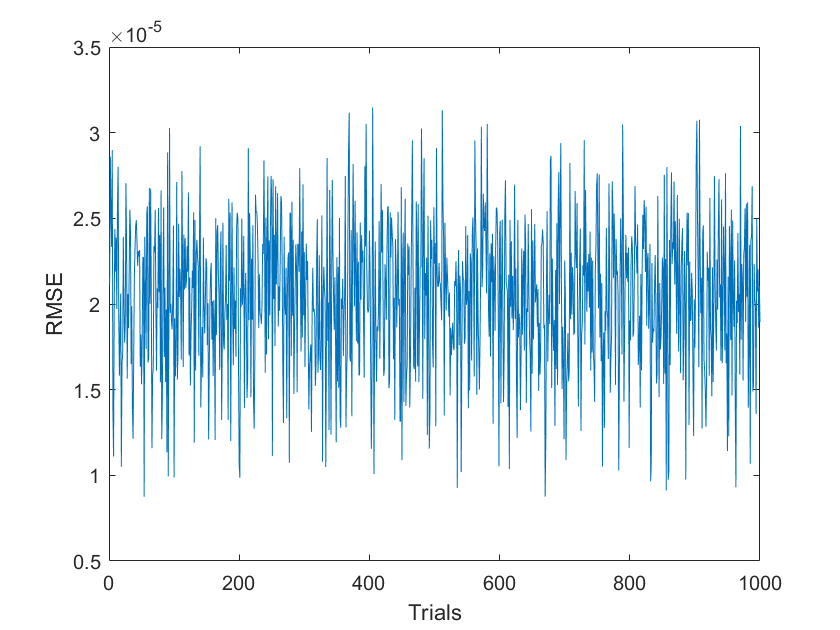
\includegraphics[width=0.7\linewidth]{error.png}
\end{figure}

而这8000个数据总共的均方根误差为$2.0871 \times 10^{-5}$,误差可接受。


\end{document}